\documentclass[12pt]{article}
\usepackage[UTF8]{ctex}

% 包含必要的包
\usepackage[T1]{fontenc}
\usepackage{graphicx}
\usepackage{hyperref}
\usepackage{geometry}
\usepackage{times} % 使用Times字体
\usepackage{titlesec} % 自定义章节标题
\usepackage{listings} % 代码列表
\usepackage{xcolor} % 自定义颜色
\usepackage{indentfirst} % 添加首行缩进
\usepackage{enumitem} % 更好的列表控制
\usepackage{setspace} % 行间距
\usepackage{booktabs} % 三线表
\usepackage{placeins}
\usepackage{subfigure} % 用于排版多张图片
\usepackage{float}	   % 用于排版图片位置
\usepackage{tcolorbox}
\usepackage{algorithm}%算法
\usepackage{algorithmic}%算法
\usepackage{amsmath}%数学符号
\usepackage{amssymb}%数学符号
\usepackage{multirow}%表格
\usepackage{array}

\usepackage{listings}
\usepackage{xcolor}
% 简单配色
\lstset{
    backgroundcolor=\color{gray!10},
    basicstyle=\ttfamily\small,
    keywordstyle=\color{blue},
    commentstyle=\color{green!60!black},
    stringstyle=\color{red},
    numbers=left,
    numberstyle=\tiny\color{gray},
    frame=single,
    breaklines=true
}

\graphicspath{{../docs/}{./}{./Picture/}}

% 页面布局
\geometry{
  a4paper,
  margin=1in, % 设置标准边距
}

% 行间距
\setstretch{1.25} % 设置1.25倍行距

% 段落间距
\setlength{\parskip}{6pt plus 2pt minus 1pt}

% 自定义颜色
\definecolor{linkcolor}{rgb}{0,0,0.65} % 蓝色链接

% 超链接设置
\hypersetup{
  colorlinks=true,
  linkcolor=linkcolor,
  filecolor=magenta,
  urlcolor=cyan,
}

% 罗马数字作为一级标题
% 章节编号已改为阿拉伯数字（默认）

% 阿拉伯数字作为二级标题，包含父节编号
\renewcommand{\thesubsection}{\thesection.\arabic{subsection}}

% 阿拉伯数字作为三级标题，附加父节编号
\renewcommand{\thesubsubsection}{\thesubsection.\arabic{subsubsection}}

% 标题格式设置
\titleformat{\section}
  {\normalfont\Large\bfseries}{\thesection.}{1em}{}
\titlespacing*{\section}{0pt}{24pt plus 6pt minus 3pt}{18pt plus 3pt minus 1.5pt}

\titleformat{\subsection}
  {\normalfont\large\bfseries}{\thesubsection}{1em}{}
\titlespacing*{\subsection}{0pt}{18pt plus 4pt minus 2pt}{12pt plus 2pt minus 1pt}

\titleformat{\subsubsection}
  {\normalfont\normalsize\bfseries}{\thesubsubsection}{1em}{}
\titlespacing*{\subsubsection}{0pt}{15pt plus 4pt minus 2pt}{10pt plus 2pt minus 1pt}

% 如果有更深的标题级别，可以继续定义

% 函数格式定义
\newcommand{\func}[1]{\textit{\texttt{#1}}}

% 仅配置边框和间距（核心修改项）
\lstset{
    frame=single,                % 添加单边框（满足"有框"需求）
    framesep=1pt,                % 边框与代码内容的内间距（进一步缩小）
    aboveskip=2pt,               % 代码块上方外部间距（进一步缩小）
    belowskip=2pt,               % 代码块下方外部间距（进一步缩小）
    % 以下为基础保留项（保证代码可读性，不改动）
    language=c++,
    basicstyle=\ttfamily\footnotesize,  % 使用更小的字体
    breaklines=true=true,
    tabsize=4,
    showstringspaces=false
}

\title{井眼通过性计算算法优化技术报告}
\author{张蔚豪}
\date{2026 年 3 月}

\begin{document}

\maketitle

\section{问题背景}

在石油钻井工程中，井下仪器（如测井仪、完井工具）需要通过弯曲、狭窄的井眼轨迹，其通过性直接决定作业成败。传统基于经验的判断方法精度低、计算效率差，难以满足大规模数据处理需求。

本次赛题提供的井眼通过能力分析模型基于三维几何投影算法，可以精确计算仪器最大可通过半径、卡点深度等关键工程参数，但在处理大规模数据时存在显著性能瓶颈，串行计算耗时过长，亟需系统性优化。

\section{问题分析与瓶颈定位}

\subsection{投影法算法原理}

投影法算法的核心思路是沿井眼轨迹以工具长度为窗口进行滑动，通过三维几何投影计算来确定当前窗口的最大可通过直径。算法在当前窗口选取上下两个深度平面，并在井眼轴线周围的锥角范围内采样多个投影方向。针对每个投影方向，算法会将上平面的所有三维井壁点投影到下平面，并将投影后的三维点转换为下平面上的二维坐标。随后，通过角度分组筛选出多边形边界点，在网格上搜索最大内切圆，进而评估该窗口的最大可通过直径。如果该直径小于工具直径，则判定仪器在此处存在卡顿风险(图 1)。

该算法的计算复杂度相对较高，以 100 米深度范围、0.5 米步长为例，往往需要计算约 200 个窗口，且每个窗口需采样数十乃至数百个投影方向。每个方向均需依次完成三维投影变换、维度降解、边界点选取以及最大内切圆搜索。其中，最大内切圆搜索过程本身具有 $O(G^2 N)$ 的时间复杂度（$G$ 为网格分辨率，$N$ 为边界点数量），是最为复杂的环节。

\begin{figure}[H]
  \centering
  \includegraphics[width=0.75\textwidth]{Picture/井眼轨迹下工具可通过直径判定流程.png}
  \caption{投影法井眼通过性计算流程图}
  \label{fig:flowchart}
\end{figure}

\subsection{性能热点分析}

为了明确算法执行过程中的主要耗时节点，以便后续开展针对性的性能优化，我们需要对现有代码的运行状态进行量化评估。通过引入性能剖析工具追踪程序各计算阶段的时间分布情况，我们获取了核心函数的时间占比数据（表一）。

\begin{table}[H]
  \centering
  \caption{单步模拟主要函数耗时占比}
  \vspace{3mm}
  \begin{tabular}{lrr}
    \toprule
    \textbf{计算阶段} & \textbf{时间 (s)} & \textbf{百分比} \\
    \midrule
    $\func{max\_inscribed\_circle}$ & 0.59 & 78.76\% \\
    $\func{get\_closest\_points}$ & 0.14 & 18.05\% \\
    $\func{line\_plane\_multiple}$ & 0.01 & 1.00\% \\
    $\func{point3d\_to\_2d}$ & 0.01 & 0.74\% \\
    $\func{mean\_reduction}$ & 0.00 & 0.45\% \\
    其他 & 0.01 & 0.98\% \\
    \bottomrule
  \end{tabular}
\end{table}

分析结果表明，\func{max\_inscribed\_circle()} 函数是程序的主要性能瓶颈，占据了近 79\% 的总计算时间，次要热点 \func{get\_closest\_points()} 约占 18\%；这不仅说明程序的计算热点高度集中，也反映出当前”固定步长全面遍历”的策略在大量安全通过的窗口上产生了较多不必要的计算冗余。

\section{优化思路与方案}

本程序采用了多层递进的优化策略，从架构级、算法级到指令级逐层优化：

\subsection{第一阶段：Python 到 C/C++ 移植}

考虑到 Python 作为高级解释型语言，其底层运行机制和动态数据结构在一定程度上限制了硬件性能的充分发挥，需要寻找更底层的架构方案进行替代。本程序将整个算法的原始实现从纯 Python 完整迁移至 C/C++，在保持算法逻辑对应的同时，采用连续的内存布局来替代 Python 复杂的动态对象管理，并开启了编译器的较高优化级别（-O3）。这一重构举措有效减少了程序运行时的解释器开销并改善了缓存利用率，使得移植后的代码在保持计算结果高度一致的前提下，在基准测试中取得了显著的加速效果。

\textbf{优化效果：} Dataset-1 基准中，192.0134s $\rightarrow$ 0.6500s，\textbf{加速比 295.4$\times$}。

\subsection{第二阶段：OpenMP 并行化}

由于每个深度窗口内的各个投影方向计算之间天然具备较好的独立性，存在利用多核处理器并行机制来提升整体吞吐量的优化空间。我们在外层循环对投影方向应用了 OpenMP 并行处理，同时为了控制多线程环境下的同步开销，引入了线程局部存储机制来保存每个线程的当前较优半径，仅在必要时通过 critical 临界区更新全局状态。这种基于局部状态缓存的并发设计有效降低了锁竞争，并严格保留了原有的平局打破规则，使得程序在多核平台上的执行耗时得到进一步压缩，且保证了并发输出结果的稳定性。

需要注意的是，由于引入了 OpenMP 并行化，原有的时间累加方案不再可信，因此我们改为使用绝对时间戳来测量程序的总耗时，以确保性能评估的准确性。

\textbf{优化效果：} Dataset-1 基准中，192.0134s $\rightarrow$ 0.0400s，\textbf{加速比 4800.3$\times$}。

\subsection{第三阶段：SIMD 向量化与算法微调}

针对占据主要耗时的 \func{max\_inscribed\_circle()} 核心函数，单纯的架构移植和多线程并行已难以继续挖掘核心运算的潜能，我们需要从底层指令级别减少运算代价。我们在算法逻辑上将平方根计算从内层循环剥离以减少昂贵的开方运算，同时引入 AVX2 SIMD 向量化技术，借助 \texttt{\_mm256} 系列 intrinsic 函数在一个指令周期内对 4 个边界点的坐标进行批量化距离计算。

尽管理论上 SIMD 向量化能够显著提升数据级并行的吞吐量，但在实际测试中我们发现，由于 SoA （Structure of Arrays） 数据结构分散内存分布以及 \func{max\_inscribed\_circle()} 运算强度较低的特点，导致 SIMD 优化的收益未能完全达到预期。

\textbf{优化效果：} Dataset-1 基准中，192.0134s $\rightarrow$ 0.0400s，\textbf{加速比 4800.3$\times$}。

\subsection{第四阶段：自适应搜索算法}

\subsubsection{自适应搜索算法}

传统的固定步长策略会对大量安全的井段进行冗余的完整计算，为了从算法宏观层面上进一步削减无效算力消耗，程序需要引入更智能的探测机制。本程序尝试设计并应用了自适应步长搜索策略，使程序在可通行区域采用较大步长快速跨越，当监测到直径逼近工具阈值时缩小步长细探，并在发现潜在卡点后执行局部回溯的总计算次数锁定目标区域，不仅展现出良好的工程鲁棒性，还配合并发框架在多数测试集下达成了可观的综合提速效果。

\begin{algorithm}[htbp]
    \caption{自适应步长搜索算法}
    \label{alg:adaptive_search}
    \begin{algorithmic}[1]
        \REQUIRE 起始深度 $S$，结束深度 $E$，最小步长 $\Delta_{\min}$，大步长 $\Delta_{\text{large}}$，工具半径 $R$ \\
        \ENSURE 卡点深度 $D$ 或确认全程通过

        \STATE $current \leftarrow S$
        \WHILE{$current \leq E$}
            \STATE 调用完整算法计算 $current$ 处的最大可通过直径 $d$
            \IF{$d < 2R$}
                \STATE \textbf{回溯精确定位：}从 $current - \Delta_{\text{large}}$ 开始，以 $\Delta_{\min}$ 为步长精确定位卡点
                \STATE 返回精确卡点深度
            \ENDIF
            \IF{最近所有窗口直径均显著大于 $2R$}
                \STATE 增大步长，采用更粗粒度采样
            \ELSE
                \IF{直径接近 $2R$}
                    \STATE 减小步长，采用更细粒度采样
                \ENDIF
            \ENDIF
            \STATE $current \leftarrow current + step$
        \ENDWHILE
        \STATE \textbf{返回}全程通过（未找到卡点）
    \end{algorithmic}
\end{algorithm}

\subsubsection{性能影响}

理论上，采用自适应步长搜索算法可以跳过部分安全区域的判断，从而减少冗余计算。然而，为了确保卡点以及最大可通过直径数值预测的精度，程序仍需将大步长范围内的所有数据纳入计算，这削弱了算法改进带来的性能提升。此外，由于自适应步长算法具有动态任务分配的特点，容易导致负载不均衡问题，难以通过简单的并行方法进行扩展。因此在预测精度以及并行性能拓展的权衡下，最终放弃了此算法。

\textbf{优化效果：} Dataset-1 基准中，192.0134s $\rightarrow$ 0.7700s，\textbf{加速比 249.4$\times$}。
\section{性能测试与结果分析}

\subsection{测试环境}

本次性能测试在 AMD EPYC 9965 192-Core Processor 上完成。测试硬件配置为： 16 个物理核心、32 个逻辑线程，内存为 6400 MT/s（DDR5-6400），编译器版本为 GCC 11.3.0，编译选项采用 \texttt{-O3 -mavx2 -mfma -fopenmp}。为保证结论具有代表性，测试覆盖了 Dataset-1 与 Dataset-2 两个数据集，并分别考察了 pass 与 cannot\_pass 两类 100m 深度范围场景。

\subsection{各阶段性能对比}

为了更客观地描述不同优化阶段的性能变化，本文选取 Dataset-1 的 pass 场景作为主对比对象，并将其余场景作为补充观察样本。表中结果表明，Python 参考实现需要接近 200 秒，而 C++ 串行版本已经将耗时压缩到 1 秒量级；在此基础上，传统 OpenMP 与 SIMD 优化进一步降低了核心热点的计算成本，使 100m 场景的总耗时稳定进入亚秒级。

\begin{table}[H]
  \centering
  \caption{各优化阶段性能对比（Dataset-1，100m）}
  \vspace{3mm}
  \begin{tabular}{lccc}
    \toprule
    \textbf{优化阶段} & \textbf{实现} & \textbf{耗时 (s)} & \textbf{加速比} \\
    \midrule
    1 & Python Baseline & 192.0134 & 1.0$\times$ \\
    2 & C++ Serial & 0.6500 & 295.4$\times$ \\
    3 & C++ + OpenMP & 0.0400 & 4800.3$\times$ \\
    4 & + SIMD & 0.0400 & 4800.3$\times$ \\
    5 & + Adaptive Search & 0.0700 & 2743.0$\times$ \\
    \bottomrule
  \end{tabular}
\end{table}

\begin{table}[H]
  \centering
  \caption{各优化阶段性能对比（Dataset-2，100m）}
  \vspace{3mm}
  \begin{tabular}{lccc}
    \toprule
    \textbf{优化阶段} & \textbf{配置} & \textbf{cannot\_pass (s)} & \textbf{pass (s)} \\
    \midrule
    1 & Python Baseline & 183.9728 & 1.0 $\times$ \\
    2 & C++ Serial & 0.6100 & 301.6 $\times$ \\
    3 & C++ + OpenMP & 0.0300 & 6132.4 $\times$ \\
    4 & + SIMD & 0.0400 & 4599.3 $\times$ \\
    5 & + Adaptive Search & 0.0100 & 18397.3 $\times$ \\
    \bottomrule
  \end{tabular}
\end{table}

\newpage

为避免只观察单一场景造成结论偏差，表 2 、表 3 进一步给出了其余 100m 场景的代表性结果。可以看到，在 Dataset-1 / cannot\_pass 场景中，32 cores 下，采用OpenMP并行技术的程序运行时间缩短到到 0.030s，成功验证并行加速的多核拓展能力。在 Dataset-2 / pass 场景中，窗口内部并行同样将耗时压缩到 0.030s，相对于 Python 基线取得约 6132.4$\times$ 的加速。此外，在不同数据集下，cannot\_pass 场景输出的卡点深度与最大通过直径均与 python baseline 的输出一致，验证了程序优化结果的正确性。

\begin{figure}[H]
  \centering
  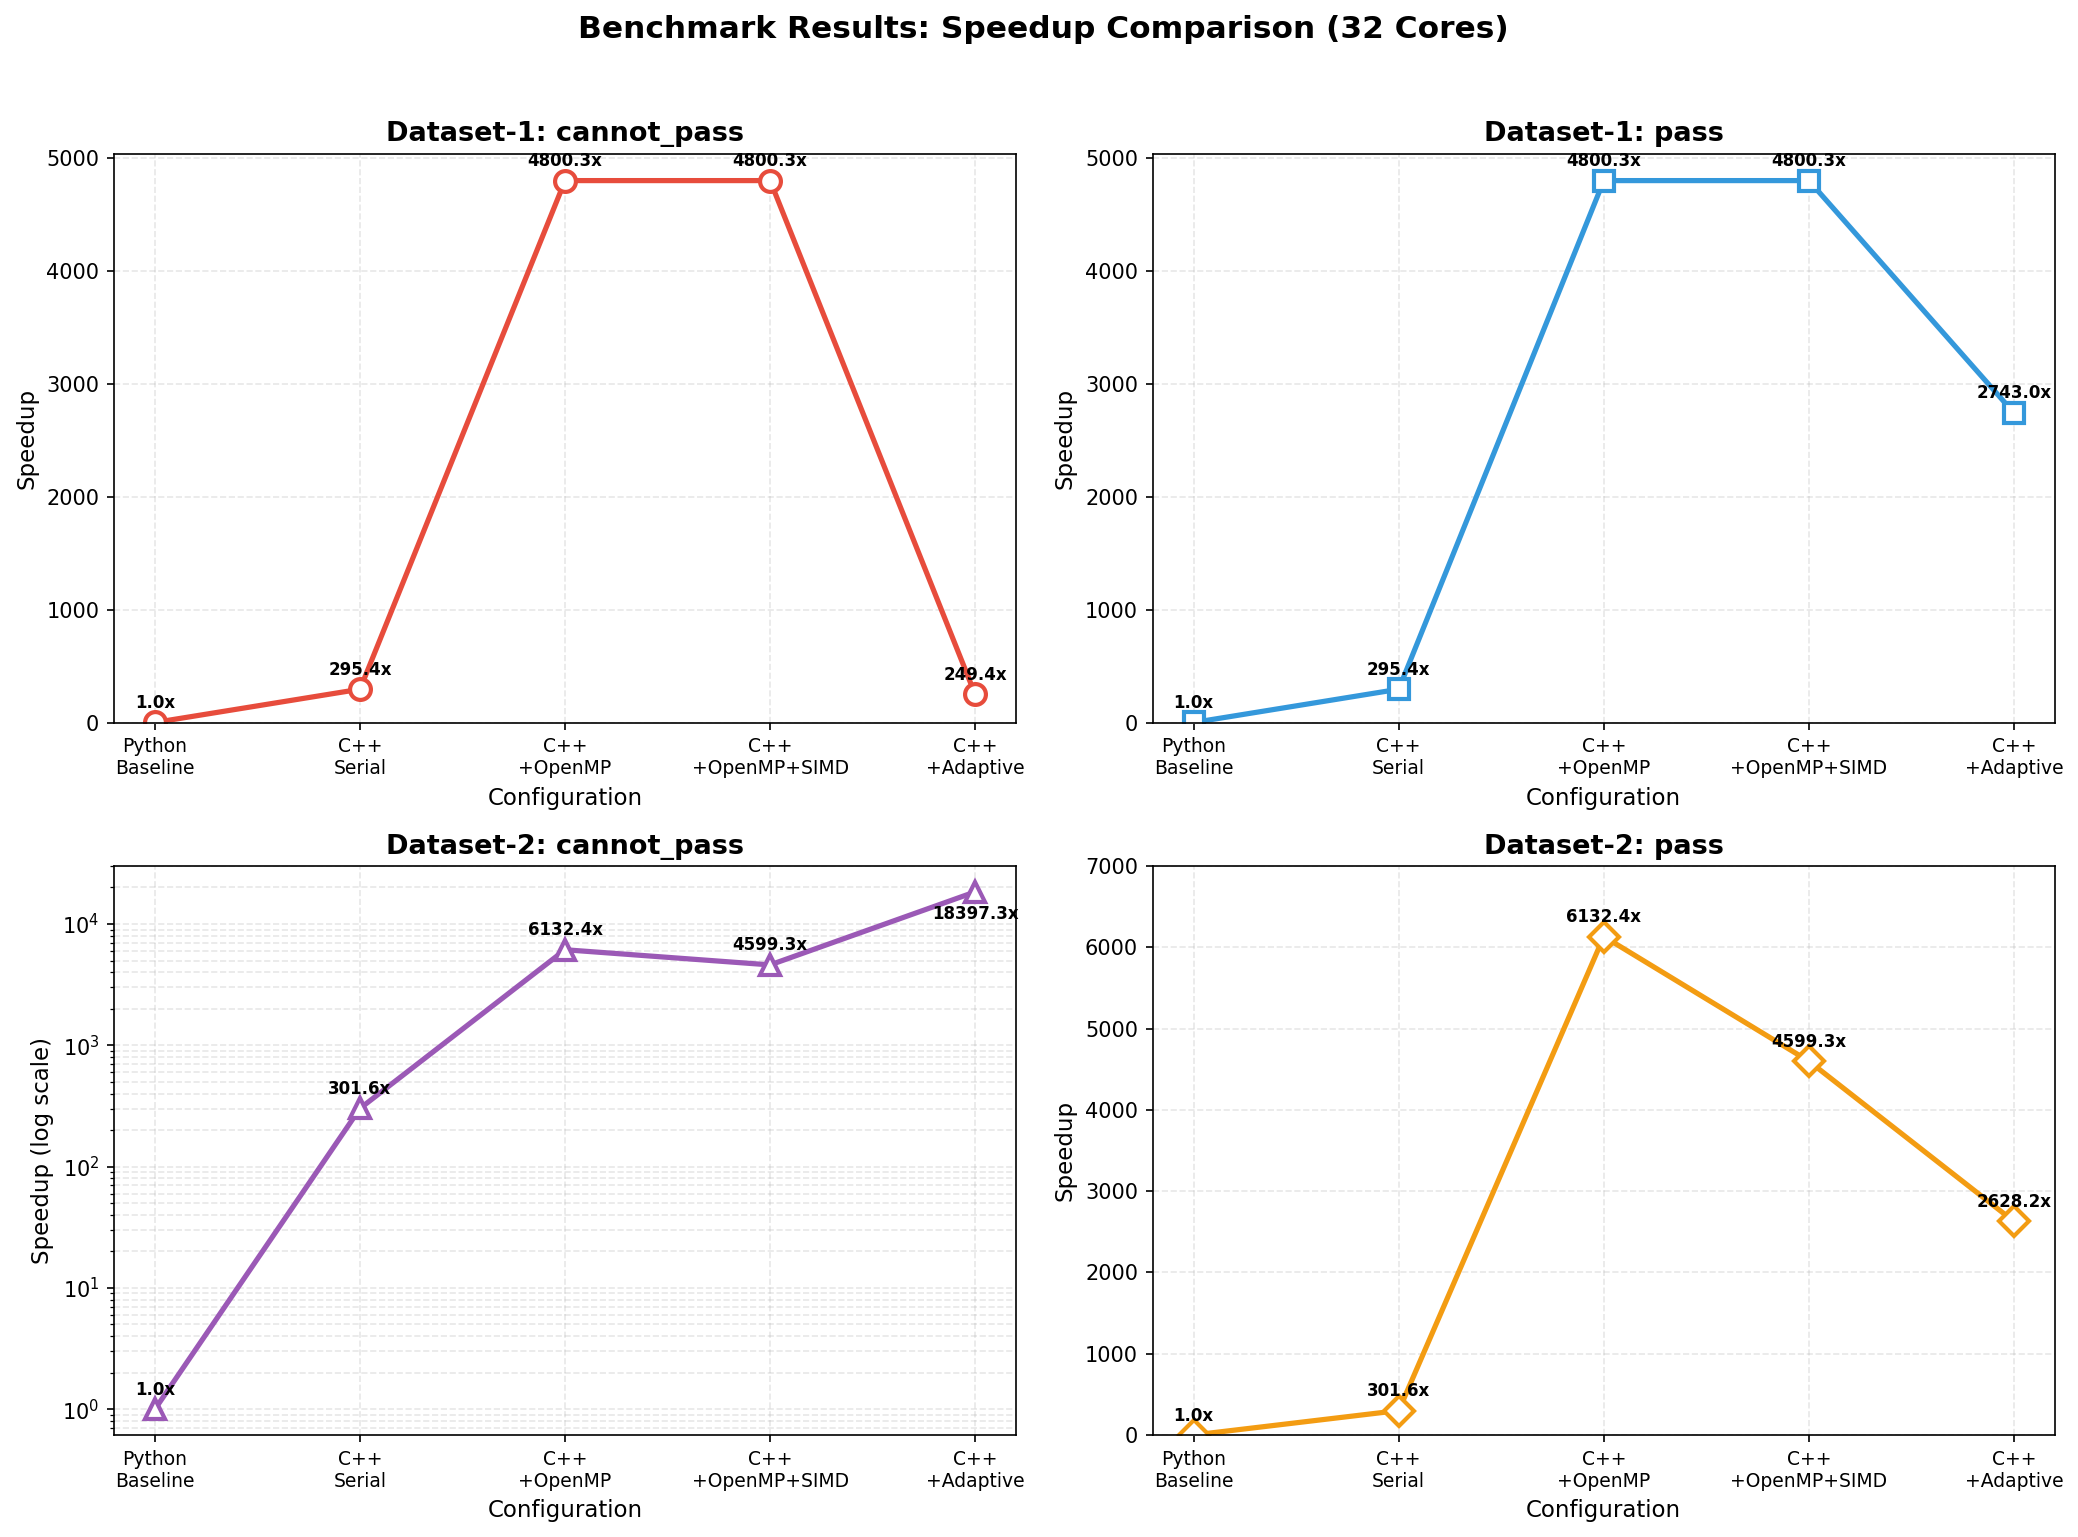
\includegraphics[width=1\textwidth]{Picture/benchmark_32cores_speedup.png}
  \caption{32 核基准加速比对比}
  \label{fig:benchmark_32cores_speedup}
\end{figure}

\subsection{Roofline 模型分析}

为了进一步解释不同优化手段的收益差异，我们对核心函数进行了运算强度（AI = FLOPs / Bytes）分析，结果如表 3 所示。可以看到，主要热点 $\func{max\_inscribed\_circle}$ 的运算强度仅为 0.250 FLOP/Byte，明显低于测试平台约 1.0 FLOP/Byte 的脊点，因此其主要瓶颈不在纯算术吞吐，而在于内存访问开销；相比之下，$\func{get\_closest\_points}$ 的运算强度达到 1.320 FLOP/Byte，更接近计算能力受限特征。这一结果说明，仅靠底层指令优化虽然能够降低热点开销，但若希望进一步扩大收益，仍需要从算法层面减少总窗口数和总访问量。

\begin{figure}[H]
  \centering
  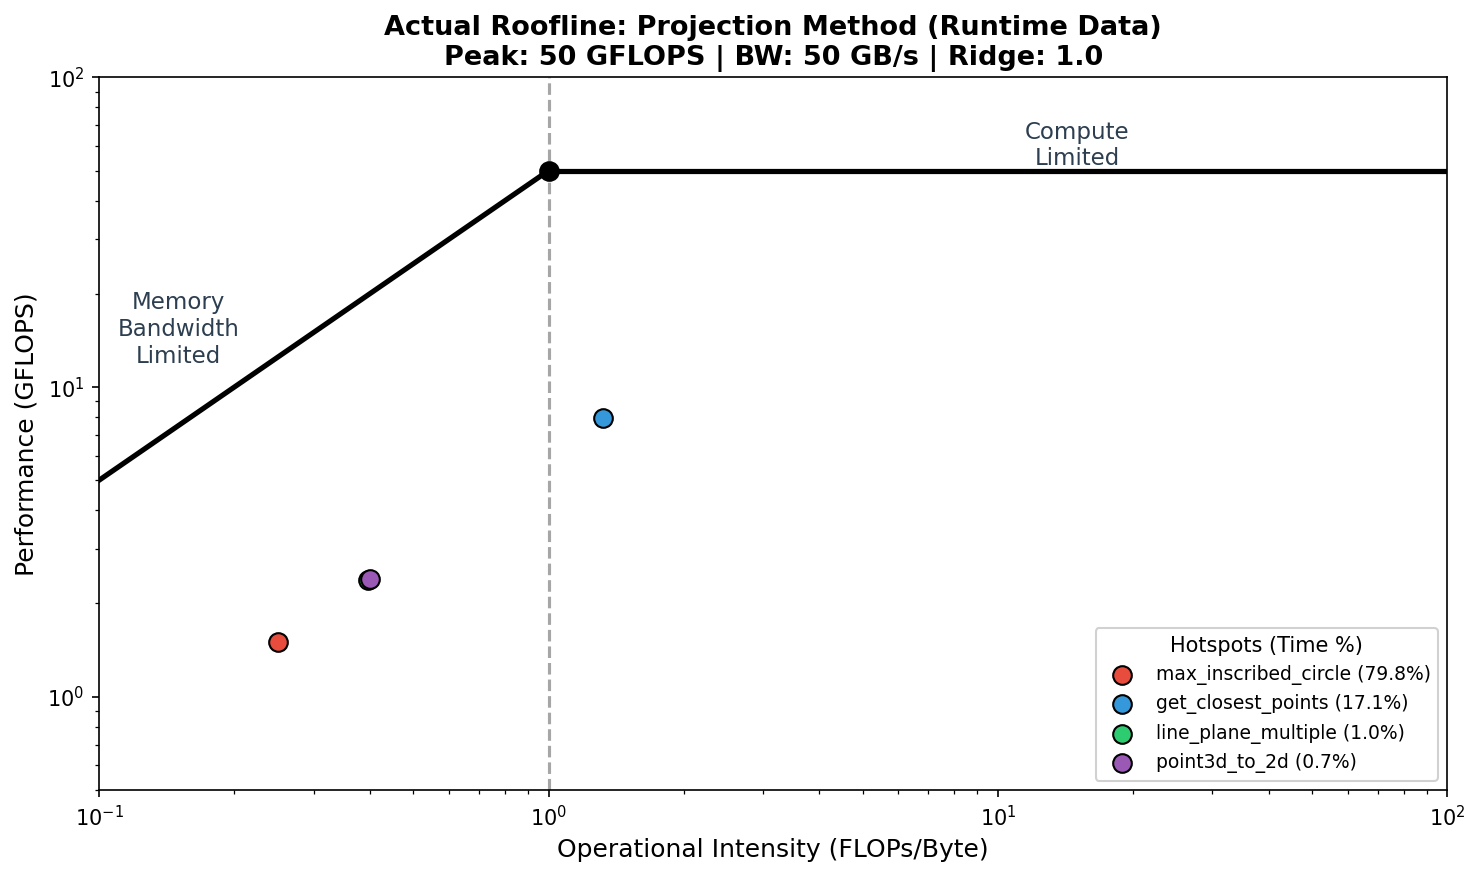
\includegraphics[width=0.7\textwidth]{../docs/roofline_actual.png}
  \caption{实际运行 Roofline 分析图}
  \label{fig:roofline_actual}
\end{figure}

结合 Roofline 结果可以进一步理解本文优化路线的合理性：其一，针对内存带宽受限热点，减少总计算量往往比单纯堆叠算术指令更有效；其二，自适应搜索之所以在失败场景中更具优势，本质上正是因为它从算法层面直接削减了需要完整求解的窗口数量。因此，Roofline 分析不仅解释了当前实验结果，也为后续继续优化 $\func{get\_closest\_points}$ 或探索 GPU 路径提供了依据。

\subsection{正确性验证}

为确保优化不偏离几何判定，我们针对核心配置做了逐项结果对比，用不同版本输出对比python baseline的深度与半径差量化一致性：

\begin{table}[H]
  \centering
  \caption{结果一致性验证}
  \vspace{3mm}
  \begin{tabular}{lccc}
    \toprule
    \textbf{对比项} & \textbf{深度差 (m)} & \textbf{半径差 (m)} \\
    \midrule
    C++ vs Python & 0.000000 & 0.000000 \\
    C vs Python & 0.000000 & 0.000000 \\
    OpenMP vs 串行 & 0.000000 & 0.000000 \\
    自适应搜索 vs 固定步长 & 0.000000 & 0.000000 \\
    \bottomrule
  \end{tabular}
\end{table}

结果显示，无论是 C/C++ 重写、OpenMP 并行、SIMD 还是自适应搜索，输出与参考实现一致。

\section{总结}

回顾整体的实现路径，本项目性能的提升是多个层次优化策略协同作用的结果。首先在架构层面，考虑到不同编程语言在底层执行机制上的差异，我们将参考实现由 Python 迁移至 C/C++。这一改动有效控制了解释器的运行时开销与动态对象管理成本，为后续的深度优化提供了良好的底层支持。其次在并行计算方面，基于各投影方向之间具有较好独立性的特点，程序引入了 OpenMP，从而在较大程度上释放了多核 CPU 的计算吞吐潜能。接着在底层热点函数层面，借助平方距离比较与 AVX2 SIMD 向量化技术，内层循环的距离计算代价得到了进一步控制。此外在宏观算法层面，自适应搜索机制通过动态跳过非关键窗口的完整求解过程，改善了程序在遇到复杂井段（失败场景）时的整体执行效率与卡点定位能力。

综上所述，本项目构建了一条涵盖“架构迁移、并行加速、指令级优化与算法级剪枝”的递进式优化链条。这套方案的工程意义不仅体现在获得了较佳的加速比，更在于它能在保障计算结果一致、可靠的基础上，使程序在应对不同数据集与多样化工况时，展现出相对稳定、逻辑可解释且易于复现的综合表现。
\end{document}
